\documentclass{article}
\usepackage[dvipsnames]{xcolor}
\usepackage[paperwidth=20cm, paperheight=4.5cm, margin = 0cm, top=0.5cm]{geometry}
\usepackage{amsmath}


\usepackage{pgf}
\usepackage{tikz}


\usetikzlibrary{arrows,automata}

\tikzstyle{source}  = [draw,circle,fill=black,thick,inner sep=0mm,minimum size=2mm]
\tikzstyle{box}  = [draw,rectangle,thick,inner sep=2mm,minimum width=8mm, minimum height=8mm]

\renewcommand{\vec}[1]{\boldsymbol{#1}}

\begin{document}
\begin{center}
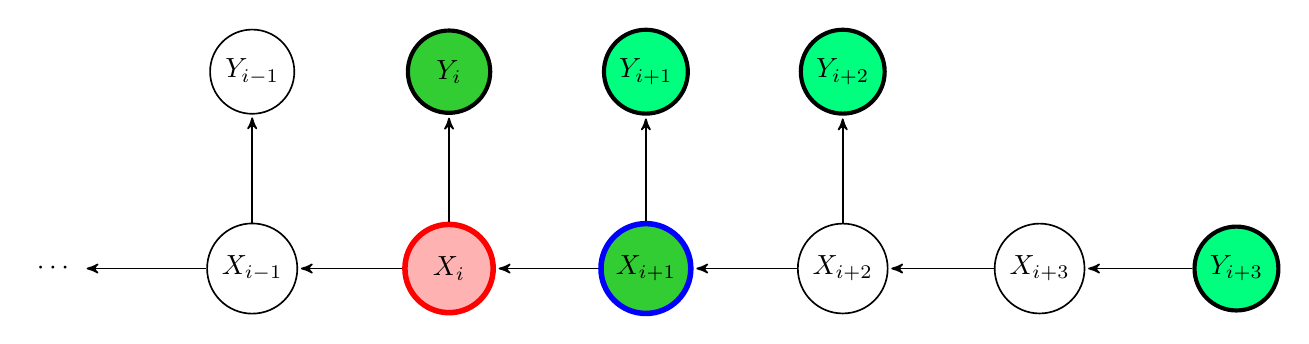
\begin{tikzpicture}[->,>=stealth',shorten >=1pt,auto,node distance=2.5cm,semithick]
                    
\node        (X0)               {$\cdots$}; 
\node[state] (X1) [right of=X0] {$X_{i-1}$}; 
\node[state, fill=red, opacity = 0.3, draw opacity=1,  draw=red, line width=2pt, text opacity =1
] (X2) [right of=X1] {$\hspace{0.5em}X_{i}\hspace{0.5em}$};                   
\node[state, fill=LimeGreen, draw=blue, line width=2pt] (X3) [right of=X2] {$X_{i+1}$};                   
\node[state] (X4) [right of=X3] {$X_{i+2}$};                   
\node[state] (X5) [right of=X4] {$X_{i+3}$};                                     

\node[state] (Y1) [above of=X1] {$Y_{i-1}$}; 
\node[state, fill=LimeGreen, draw=black, opacity=1, line width=1.5pt] (Y2) [above of=X2] {$\hspace{0.5em}Y_{i}\hspace{0.5em}$}; 
\node[state, fill=SpringGreen, text opacity=1, draw opacity=1, line width=1.5pt] (Y3) [above of=X3] {$Y_{i+1}$}; 
\node[state, fill=SpringGreen, text opacity=1, draw opacity=1, line width=1.5pt] (Y4) [above of=X4] {$Y_{i+2}$}; 
\node[state, fill=SpringGreen, text opacity=1, draw opacity=1, line width=1.5pt] (Y5) [right of=X5] {$Y_{i+3}$}; 
	
\path
             (X1) edge  (X0)  
	(X2) edge  (X1)
	(X3) edge  (X2)
	(X4) edge  (X3)
	(X5) edge  (X4);
\path	
	(X1) edge  (Y1)
	(X2) edge  (Y2)
	(X3) edge  (Y3)
	(X4) edge  (Y4)
	(Y5) edge  (X5);
\end{tikzpicture}
\end{center}

\end{document}
